\chapter{Limit Laws, the Squeeze Theorem, and the Intermediate Value Theorem}

\section{Limits Rules}
In the last chapter, you found limits by staring at graphs and tables.
That works, but it is slow, and graphs can fool you. A few simple rules,
the limit laws, let you compute limits of complicated functions by breaking
them into simple pieces.

The following laws are true given that \textit{c} is a constant, $\lim_{x\to a} 
f(x) $ exists, and $\lim_{x\to a} g(x) $ exists.

\begin{enumerate}
    \item Sum Law $\lim_{x\to a} \left[f(x) + g(x) \right] = \lim_{x\to a} f(x) 
    + \lim_{x\to a} g(x)$
    \item Difference Law $\lim_{x\to a} \left[f(x) - g(x) \right] = 
    \lim_{x\to a} f(x) - \lim_{x\to a} g(x)$
    \item Constant Multiple Law $\lim_{x\to a} \left[\textit{c}f(x) \right] = 
    \textit{c} \cdot \lim_{x\to a} f(x) $
    \item Product Law $\lim_{x\to a} \left[f(x)g(x) \right] = \lim_{x\to a}f(x) 
    \cdot \lim_{x\to a} g(x)$
    \item Quotient Law $\lim_{x\to a} \frac{f(x)}{g(x)} = \frac{\lim_{x\to a} 
    f(x)}{\lim_{x\to a} g(x)}$ given that $\lim_{x\to a} g(x) \neq 0$
\end{enumerate}
These laws are fairly obvious --- the limit of the sum of two functions is equal to 
the sum of the limits of each function individually. The only tricky one is the 
last: The limit of the quotient of two functions is equal to the quotient of the 
limits if and only if the limit of the function in the denominator does not equal 
zero. This makes sense, as we know dividing by zero yields an undefined result. 

Let us practice applying these laws to evaluate the limits of the functions f(x), 
shown in blue below, and g(x), shown in red below:

$f(x) = \begin{cases}
    -x^2+3, \text{ if } x \leq 0\\
    -x, \text{ if } x > 0
\end{cases}$

$g(x) = \begin{cases}
   x^2+1, \text{ if } x < 1 \\
    (x-2)^2, \text{ if } x \geq 1
\end{cases}$

\begin{figure}[H]
\centering
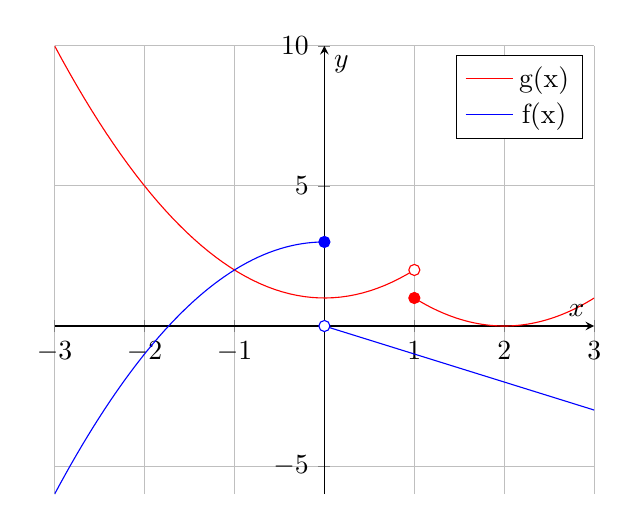
\begin{tikzpicture}
    \begin{axis}[
        grid,
        axis lines = center,
        xlabel = \(x\),
        ylabel = {\(y\)},
        ]
    \addplot [
    domain=-3:1,
    samples=50,
    color=red,
    ]
    {x^2+1};
    \addlegendentry{g(x)};
    \addplot[
    domain=-3:0,
    samples=50,
    color=blue,
    ]
    {-x^2+3};
    \addlegendentry{f(x)};
    \addplot[
    domain=1:3,
    samples=50,
    color=red,
    ]
    {(x-2)^2};
    \addplot[mark=*,fill=red,draw=red] coordinates{(1,1)};
    \addplot[mark=*,fill=white,draw=red] coordinates{(1,2)};
    
    \addplot[mark=*,fill=blue,draw=blue] coordinates{(0,3)};
    \addplot[mark=*, fill=white,draw=blue] coordinates{(0,0)};
    \addplot[
    domain=0:3,
    samples=50,
    color=blue,
    ]
    {-x};
    \end{axis}
\end{tikzpicture}
\caption{Graphs of the piecewise functions $f(x)$ and $g(x)$}
\end{figure}
We can use these laws to evaluate limits involving $f(x)$ and $g(x)$ (shown on the 
graph above). Here are some examples:
Use the graphs of f(x) and g(x) given above to evaluate each limit, if it exists. 
If the limit does not exist, explain why. Two examples are given first:

\textbf{Example 1}: Evaluate $\lim_{x\to0} f(x) \cdot g(x)$

\textbf{Solution 1}: From the Product Law, we know that:
$$\lim_{x\to0} f(x) \cdot g(x) = \lim_{x\to0}f(x) \cdot \lim_{x\to0} g(x)$$

Looking at the graph, we can see that 
$$\lim_{x\to0}g(x) = 1$$ 

and there is a discontinuity in $f(x)$ at $x=0$. Therefore, 
$$\lim_{x\to0}f(x) = \text{DNE}$$

Substituting this, we get: 
$$\lim_{x\to0}f(x) \cdot \lim_{x\to0} g(x) = \text{DNE} \cdot 1 = \text{DNE}$$

Therefore, \textit{the limit does not exist}. 

\textbf{Example 2}: Evaluate $\lim_{x\to2}f(x) - g(x)$

\textbf{Solution 2}: Applying the Difference Law, we see that:

$$\lim_{x\to2}[f(x) - g(x)] = \lim_{x\to2}f(x) - \lim_{x\to2}g(x)$$

Examining the graph, we see that 
$$\lim_{x\to2}f(x) = -2$$ 

and 
$$\lim_{x\to2}g(x) = 0$$

Substituting these values, we get:

$$\lim_{x\to2}f(x) - g(x) = -2 - 0 = -2$$

\begin{Exercise}
    [title = Limits Practice 6, label=limits6_ivt]
\begin{enumerate}
    \item $\lim_{x\to-3} \frac{f(x)}{g(x)}$
    \item $\lim_{x\to2}\left[f(x) + 5g(x)\right]$
    \item $\lim_{x\to-1} \frac{3g(x)}{f(x)}$
    \item $\lim_{x\to0}f(x) \cdot 5g(x)$
    \item $\lim_{x\to-1} f(x) - 3g(x) $
\end{enumerate}
\vspace{40mm}
\end{Exercise}
\begin{Answer}
    [ref=limits6_ivt]
    \begin{enumerate}
        \item From the quotient law, we know that:
        $$\lim_{x\to-3}\frac{f(x)}{g(x)}=\frac{\lim_{x\to-3}f(x)}{\lim_{x\to-3}g(x)}$$\\
        From the graph (or the formulas), we see that:
        $$\lim_{x\to-3}f(x) = -(-3)^2 + 3 = -6$$ \\
        and that:
        $$\lim_{x\to-3}g(x) = (-3)^2 + 1 = 10$$ \\
        Substituting these values, we get:
        $$\lim_{x\to-3}\frac{f(x)}{g(x)}=\frac{-6}{10} = -\frac{3}{5}$$
        \item From the Sum Law, we know that: 
        $$\lim_{x\to2}\left[f(x) + 5g(x)\right]=\lim_{x\to2}f(x) + \lim_{x\to2}5g(x)$$\\
        and applying the Constant Multiple Law, we see that: 
        $$\lim_{x\to2}\left[f(x) + 5g(x)\right]=\lim_{x\to2}f(x) + 5\lim_{x\to2}g(x)$$\\
        Examining the graph of f(x) and g(x), we can determine that 
        $$\lim_{x\to2}f(x) = -2$$ \\
        and 
        $$\lim_{x\to2}g(x) = 0$$\\ 
        Substituting these values, we get: 
        $$\lim_{x\to2}\left[f(x) + 5g(x)\right]=-2 + 5 \cdot 0 = -2$$\\
        \item From the quotient law, we see that: 
        $$\lim_{x\to-1} \frac{3g(x)}{f(x)}=\frac{\lim_{x\to-1}3g(x)}{\lim_{x\to-1}f(x)}$$\\ 
        Applying the Constant Multiple Law, we get: 
        $$\lim_{x\to-1} \left[\frac{3g(x)}{f(x)}\right]=\frac{3\lim_{x\to-1}g(x)}{\lim_{x\to-1}f(x)}$$\\ 
        From the graph, we see that: 
        $$\lim_{x\to-1}f(x) = 2$$\\
        and 
        $$\lim_{x\to-1}g(x) = 2$$\\ 
        Substituting, we get: 
        $$\lim_{x\to-1} \left[\frac{3g(x)}{f(x)}\right]=\frac{3 \cdot 2}{2}=3$$\\
        \item Applying the Product and Constant Multiple Laws, we get: 
        $$\lim_{x\to0}\left[f(x) \cdot 5g(x)\right] = \lim_{x\to0}f(x) \cdot 5 \cdot \lim_{x\to0}g(x)$$\\
        Examining the graphs, we see that $\lim_{x\to0}f(x)$ does not exist and 
        $\lim_{x\to0}g(x) = 1$. Because $\lim_{x\to0}f(x)$ does not exist, 
        $\lim_{x\to0}f(x) \cdot 5 \cdot \lim_{x\to0}g(x)$ also does not exist. 
        \item Applying the Difference and Constant Multiple Laws, we see that: 
        $$\lim_{x\to-1} \left[f(x) - 3g(x)\right] =\lim_{x\to-1}f(x) - 3 \cdot \lim_{x\to-1}g(x)$$ \\
        Examining the graphs, we see that: 
        $$\lim_{x\to-1}f(x) = 2$$\\ 
        and 
        $$\lim_{x\to-1}g(x) = 2$$\\ 
        Substituting, we get that: 
        $$\lim_{x\to-1} \left[f(x) - 3g(x)\right] =2 - 3 \cdot 2 = 2-6 = -4$$\\
    \end{enumerate}
\end{Answer}


Recall that exponents represent repeated multiplication. Therefore, if we apply the 
Product Law multiple times, we obtain the Power Law for limits:
\begin{enumerate}
    \setcounter{enumi}{5}
    \item Power Law $\lim_{x \to a} \left[ f(x) \right]^n = \left[
    \lim_{x \to a} f(x) \right]^n$ where $n$ is a positive integer
\end{enumerate}
There are two special limits that will be useful to us and are intuitively 
obvious, but we will not formally prove here.  
\begin{enumerate}
    \setcounter{enumi}{6}
    \item $\lim_{x\to a} \textit{c} = \textit{c}$
    \item $\lim_{x\to a} x = a$
\end{enumerate}
Combining Law 8 with the Power Law, we find that:
\begin{enumerate}
\setcounter{enumi}{8}
    \item $\lim_{x\to a} x^n = a^n$
\end{enumerate}
And similarly, for square roots:
\begin{enumerate}
    \setcounter{enumi}{9}
    \item $\lim_{x\to a} \sqrt[n]{x} = \sqrt[n]{a}$ (if n is even, we assume $a > 0$)
\end{enumerate}

Direct substitution property: If $f$ is a polynomial or rational function and $a$ 
is in the domain for $f$, then $$\lim_{x \to a}f(x) = f(a)$$

Often, rational functions can be simplified. In the limits chapter, we computed the
limit by simplifying $f(x) = \frac{3x^2-8x-3}{x-3}$ to the simpler $g(x) = 3x+1$. 
This is a valid strategy because $\frac{3x^2-8x-3}{x-3} = 3x+1$ when $x \neq 3$. 
Remember: a limit describes how a function behaves \textit{as it approaches} $a$, 
not its value/behavior when $x$ \textit{actually equals} $a$. This reveals the 
following useful rule: 
$$\text{If } f(x)=g(x) \text{ when } x \neq a \text{, then } 
\lim_{x \to a}f(x) = \lim_{x \to a}g(x) \text{, provided the limit exists.}$$

\section{Squeeze Theorem}

\index{Squeeze Theorem}The Squeeze Theorem states that if $f(x) \leq g(x) \leq h(x)$ when $x$ is near $a$ 
(except at $a$) and $$\lim_{x \to a}f(x)=\lim_{x \to a}h(x) = L$$ then $$\lim_{x 
\to a}g(x) = L$$

In other words, if $g(x)$ is between $f(x)$ and $h(x)$ near $a$, and $f$ and $h$ have the 
same limit, $L$, then the limit of $g$ must also be $L$. 

\textbf{Example}: Let us examine the graph of $g(x) = x^2\sin{\frac{1}{x}}$ and determine $\lim_{x \to 
0}g(x)$:

\begin{figure}[H]
\centering
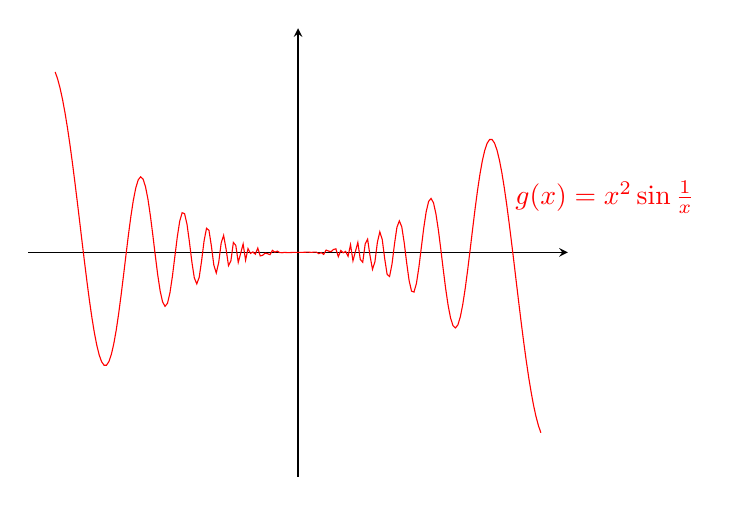
\begin{tikzpicture}
    \begin{axis}[clip=false,
    xmin=-.1, xmax=.1,
    ymin=-.01, ymax=0.01,
    axis lines=middle,
    xtick=\empty,
    ytick=\empty,
    ]
     \addplot[domain=-.09:0.09, red, samples=200]{(x^2)*sin(deg(1/x))}
     node[right, pos=0.92]{$g(x)=x^2\sin{\frac{1}{x}}$}; 
     %\addplot[domain=-.09:0.09, blue, samples=50]{x^2}
     %node[right, pos=0.95]{$g(x)=x^2$};
     %\addplot[domain=-.09:0.09, black, samples=50]{-x^2}
     %node[right, pos=1]{$h(x)=-x^2$};
    \end{axis}
\end{tikzpicture}
\caption{Graph of $g(x) = x^2\sin{\frac{1}{x}}$}
\end{figure}

\textbf{Solution}: Because $\sin{\frac{1}{x}}$ is undefined at $x=0$, we cannot 
compute the limit directly. However, from examining the graph, we can guess 
that $\lim_{x \to 0} g(x) = 0$. Feel free to confirm this with your calculator. 
We need to choose two functions: one that is larger than $g(x)$ near $x = 0$ 
and one that is smaller. Since $|\sin{\frac{1}{x}}|\leq 1$ (when $x \neq 0$), 
then $$|x^2 \sin{\frac{1}{x}}| \leq x^2$$ and $$-x^2 \leq x^2 \sin{\frac{1}{x}} 
\leq x^2$$

Let us confirm this by plotting $f(x)=-x^2$, $g(x)$, and $h(x)=x^2$ on the same 
graph:

\begin{figure}[H]
\centering

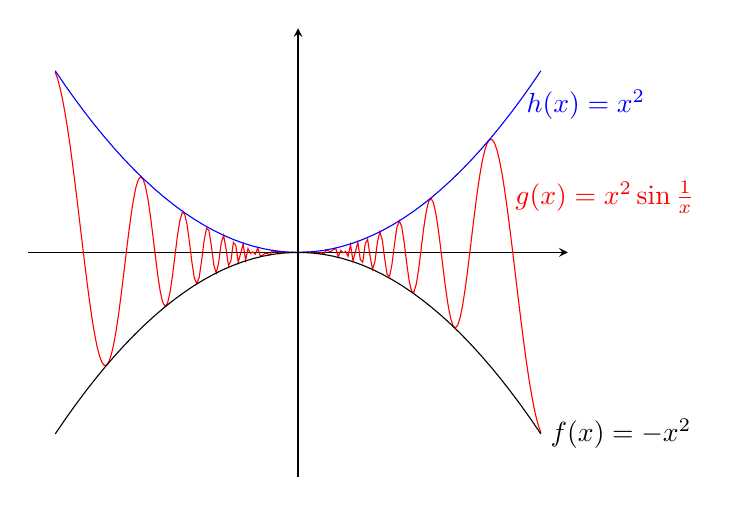
\begin{tikzpicture}
    \begin{axis}[clip=false,
    xmin=-.1, xmax=.1,
    ymin=-.01, ymax=0.01,
    axis lines=middle,
    xtick=\empty,
    ytick=\empty,
    ]
     \addplot[domain=-.09:0.09, red, samples=200]{(x^2)*sin(deg(1/x))}
     node[right, pos=0.92]{$g(x)=x^2\sin{\frac{1}{x}}$}; 
     \addplot[domain=-.09:0.09, blue, samples=50]{x^2}
     node[right, pos=0.95]{$h(x)=x^2$};
     \addplot[domain=-.09:0.09, black, samples=50]{-x^2}
     node[right, pos=1]{$f(x)=-x^2$};
    \end{axis}
\end{tikzpicture}
\caption{Squeeze Theorem example}
\end{figure}

As you can see, when $x$ is near $0$, $f(x) \leq g(x) \leq h(x)$. Because $f(x)$ 
and $h(x)$ are both polynomials, their limits are straightforward: $$\lim_{x \to 
0}-x^2 = 0 \text{ and } \lim_{x \to 0}x^2 = 0$$

Then, by the Squeeze Theorem, we can say that: $$\lim_{x \to 0}x^2\sin{\frac{1}{x}}
=0$$

\subsection{Squeeze Theorem Practice}

\begin{Exercise}
[title=Squeeze Theorem 1, label=squeeze1]
    Use the Squeeze Theorem to show that $\lim_{x \to 0}\sqrt{x^3 + x^2}
    \cos{\frac{1}{x}} = 0$. Illustrate by graphing the functions you define as 
    $f$, $g$, and $h$ on the same plot.
    \vspace{100mm}
\end{Exercise}
\begin{Answer}
    [ref=squeeze1]
    Let $f(x) = -\sqrt{x^3+x^2} \text{ and } h(x) = \sqrt{x^3+x^2}$. Near $0$, 
    $f(x) \leq \sqrt{x^3 + x^2}\cos{\frac{1}{x}} \leq h(x)$. Additionally, 
    $\lim_{x \to 0}f(x) = \lim_{x \to 0}h(x) = 0$. Therefore, by the Squeeze 
    Theorem, we can state that $\lim_{x \to 0}\sqrt{x^3 + x^2}\cos{\frac{1}{x}} 
    = 0$. Plotting all three functions, we can confirm our answer:

  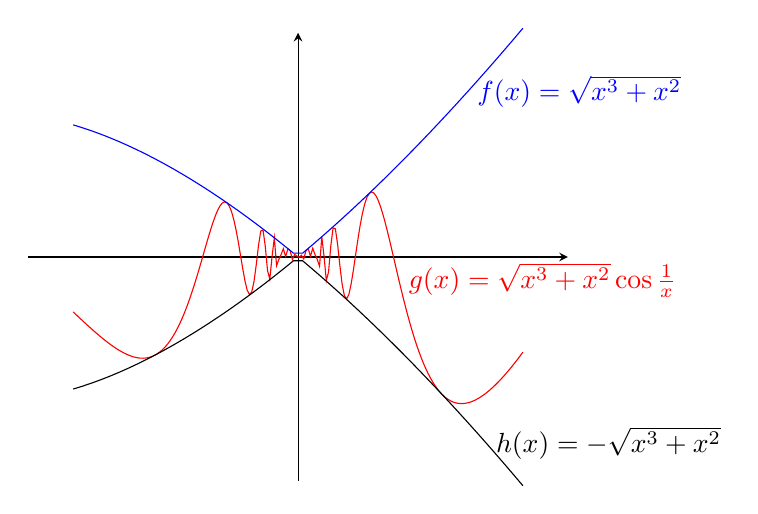
\begin{tikzpicture}
    \begin{axis}[clip=false,
    xmin=-.6, xmax=.6,
    ymin=-.6, ymax=0.6,
    axis lines=middle,
    xtick=\empty,
    ytick=\empty,
    ]
    \addplot[domain=-0.5:0.5, red, samples=200]{sqrt(x^3+x^2)*cos(deg(1/x))}
    node[right, pos=0.83]{$g(x)=\sqrt{x^3+x^2}\cos{\frac{1}{x}}$};
    \addplot[domain=-0.5:0.5, blue, samples=50]{sqrt(x^3+x^2)}
    node[right, pos=0.85]{$f(x)=\sqrt{x^3+x^2}$};
    \addplot[domain=-0.5:0.5, black, samples=50]{-sqrt(x^3+x^2)}
    node[right, pos=0.9]{$h(x) = -\sqrt{x^3+x^2}$};
    \end{axis}
\end{tikzpicture}  
\end{Answer}

\begin{Exercise}
    [title=Squeeze Theorem 2, label=squeeze2]
    If $2x+3 \leq f(x) \leq x^2-2x+7$ for $x \geq 0$, find $\lim_{x \to 2}f(x)$
    \vspace{40mm}
\end{Exercise}
\begin{Answer}
    [ref=squeeze2]
    The question tells us that the function in question, $f(x)$, is between 
    two other functions. $\lim_{x \to 2}2x+3 = 2(2)+3 = 7$ and $\lim_{x \to 2} 
    x^2 - 2x + 7 = 2^2 - 2(2) + 7 = 7$. Since the limits are equal, by Squeeze 
    Theorem we can also know that $\lim_{x \to 2}f(x) = 7$.
\end{Answer}

\begin{Exercise}
    [title= Squeeze Theorem 3, label=squeeze3]
    Prove that $\lim_{x \to 0^+}\sqrt{x}e^{\sin{\frac{\pi}{x}}} = 0$
    \vspace{40mm}
\end{Exercise}

\begin{Answer}
    [ref=squeeze3]
    Note that we can only evaluate the limit from the right, as the domain for this 
    function is $x \geq 0$. Since the range of the sine function is $[-1,1]$, we 
    can state that $$-1 \leq \sin{\frac{\pi}{x}} \leq 1$$ 
    and therefore $$\frac{1}{e} \leq e^{\sin{\frac{\pi}{x}}} \leq e$$. Because 
    we assume the positive root, it is also true that $$\frac{\sqrt{x}}{e} \leq 
    \sqrt{x}e^{\sin{\frac{\pi}{x}}} \leq \sqrt{x}e$$. Taking the limits of the 
    border functions, we see that $$\lim_{x \to 0^+}\frac{\sqrt{x}}{e} = \lim_{x 
    \to 0^+}\sqrt{x}e = 0$$ Therefore, $$\lim_{x \to 0^+}\sqrt{x}e^{\sin{\frac{\pi}
    {x}}}=0$$
\end{Answer}


\section{Intermediate Value Theorem}\index{Intermediate Value Theorem}
When considering functions that are continuous on a closed interval, the 
Intermediate Value Theorem can help us: Given a function, $f(x)$, that is 
continuous on the closed interval $\left[a, b\right]$ and $f(a) \neq f(b)$, 
there is at least one number $c$ such that $f(c) = N$, where $N$ is any number 
between $f(a)$ and $f(b)$. The theorem is illustrated in figures \ref{fig:IVT1} 
and \ref{fig:IVT2}:

\begin{figure}[hbtp]
\centering
\begin{tikzpicture}
    \begin{axis}[
    axis lines = left, 
    xlabel = \(x\), 
    ylabel=\(f(x)\), 
    ymin=0, 
    xtick=\empty,
    ytick=\empty,
    extra y ticks={2.5,6.5, 4.3},
    extra y tick labels={$f(a)$, $f(b)$, $N$},
    extra x ticks = {0.265, 3.75, 3.465},
    extra x tick labels = {$a$, $b$, $c$}
    ]
        \addplot[domain = 0:4, samples =50, color=blue]{(x-1.8)^3-2*(x-1.8)+3};
        \addplot[domain=0:3.75, color=green]{6.5};
        \addplot[samples=50,domain=0:6,green] coordinates {(3.75,0)(3.75,6.5)};
        \addplot[domain = 0:0.265, samples = 50, color=green]{2.5};
        \addplot[samples=50,domain=0:6,green] coordinates {(0.265,0)(0.265, 2.5)};
        \addplot[domain=0:3.465, color=red]{4.3};
        \addplot[domain=0:6, red] coordinates{(3.465,0)(3.465,4.3)};
    \end{axis}
\end{tikzpicture}
\caption{An example where one solution satisfies the Intermediate Value Theorem}
\label{fig:IVT1}
\end{figure}

\begin{figure}[H]
\centering
\begin{tikzpicture}
    \begin{axis}[
    axis lines = left, 
    xlabel = \(x\), 
    ylabel=\(f(x)\), 
    ymin=0,
    xtick=\empty,
    ytick=\empty,
    extra y ticks={2.5,6.5, 3.2},
    extra y tick labels={$f(a)$, $f(b)$, $N$},
    extra x ticks = {0.265, 3.75, 0.445, 1.7, 3.25},
    extra x tick labels = {$a$, $b$, $c_1$, $c_2$, $c_3$}
    ]
        \addplot[domain = 0:4, samples =50, color=blue]{(x-1.8)^3-2*(x-1.8)+3};
        \addplot[domain=0:3.75, color=green]{6.5};
        \addplot[samples=50,domain=0:6,green] coordinates {(3.75,0)(3.75,6.5)};
        \addplot[domain = 0:0.265, samples = 50, color=green]{2.5};
        \addplot[samples=50,domain=0:6,green] coordinates {(0.265,0)(0.265, 2.5)};
        \addplot[samples=50, red, domain=0:3.25]{3.2};
        \addplot[samples=50,domain=0:6,red] coordinates {(0.445,0)(0.445, 3.2)};
        \addplot[samples=50,domain=0:6,red] coordinates {(1.7,0)(1.7, 3.2)};
        \addplot[samples=50,domain=0:6,red] coordinates {(3.25,0)(3.25, 3.2)};
    \end{axis}
\end{tikzpicture}
\caption{An example where more than one solution satisfies the Intermediate 
Value Theorem}
\label{fig:IVT2}
\end{figure}

Logically, we can think of the IVT this way: If a function is continuous on a 
closed interval, there are no gaps or breaks. If there are no gaps or breaks, 
then the function must pass through the line $y=N$, since it cannot jump over 
the line. Calculators and computers find roots this way: if $f$ is negative at one
end of an interval and positive at the other, a root must lie between, so
they cut the interval in half and keep the half where the sign still
changes. You will write this \emph{bisection method} yourself in the
root-finding chapter.

\textbf{Example}: Show that there is at least one root of the equation $2x^3 - 
6x^2 + 3x - 1 = 0$ between $x = 2$ and $x = 3$.

\textbf{Solution}: For IVT to apply, we must first check that the function is 
continuous on the closed interval $x \in \left[2, 3\right]$. We define $f(x) =
2x^3-6x^2+3x-1$, which is continuous everywhere, because it is a polynomial 
function. \textit{For more complex functions, always be sure to check the 
endpoints of an interval, since IVT only applies on closed intervals of 
continuity}. We will take $a = 2$, $b = 3$, and $N = 0$. We find the values of 
$f(x)$ at the endpoints: 

$$f(2) = 2(2)^3 - 6(2)^2 + 3(2) - 1 = 16 - 24 + 6 - 1 = -3$$
$$f(3) = 2(3)^3 - 6(3)^2 + 3(3) - 1 = 54 - 54 + 9 - 1 = 8$$

Therefore, $f(2)<0<f(3)$ and according to IVT, there must exist some $c$ such 
that $f(c) = 0$ and there is a root to the equation in the interval $x \in 
\left(2, 3\right)$.

\begin{Exercise}
    [title=Intermediate Value Theorem Practice, label=IVTPrac]
    Use the IVT to show there is a solution the given equation on the stated 
    interval:\
    \begin{enumerate}
        \item $2x^4+x-12=0 \text{ , } \left(1, 2\right)$
        \item $\ln(x)=3x-4\sqrt{x}\text{ , } \left(2, 3\right)$
        \item $2\sin{x} = 3x^2-2x\text{ , } \left(1, 2\right)$
        \vspace{75mm}
    \end{enumerate}
\end{Exercise}
\begin{Answer}
    [ref=IVTPrac]
    \begin{enumerate}
        \item define $f(x)=2x^4+x-12$, $a=1$, $b=2$, and $N=0$. Calculate 
        $f(a)$ and $f(b)$:
        $$f(1)=-9 \text{ and } f(2)=22$$ \\
        Since $f(x)$ is a polynomial, it is continuous on the interval $x\in
        \left[1, 2\right]$ and we see that $f(a) < 0 < f(b)$. Therefore, there 
        exists some $c \in \left[1, 2\right]$ such that $f(c)=0$.\
        
        \item First, we can rearrange the equation we are considering and 
        define $f(x) = \ln{x} - 3x + 4\sqrt{x}$, and realize we are looking for 
        values where $f(x) = 0$. Both $\ln{x}$ and $\sqrt{x}$ are only continuous 
        for $x > 0$. The interval we are interested in, $x \in \left[2, 
        3\right]$, is in the domain of continuity for both $\ln{x}$ and 
        $\sqrt{x}$. Defining $a = 2$, $b = 3$, and $N = 0$, we find that $f(a) 
        = 0.35 > N > -0.973 = f(b)$. Since $N \in \left[f(b), f(a)\right]$, 
        there must exist some $c$ such that $f(c) = N = 0$ and there is a 
        solution to the equation $\ln{x} = 3x - 4\sqrt{x}$ on the interval $x 
        \in \left(2, 3\right)$.
        
        \item Similar to above, define $f(x) = 2\sin{x} - 3x^2 + 2x$, $a = 1$, 
        $b = 2$, and $N = 0$. Calculate that $f(a) = 0.683$ and $f(b) = -6.181$. 
        Since $f(x)$ is continuous on the interval $ x \in \left[1, 2\right]$ 
        and $f(b) < N < f(a)$, there exists some $c \in \left(1, 2 \right)$ 
        such that $f(c) = 0$. Therefore, there is a solution to $2\sin{x} =
        3x^2 - 2x$ on the interval $ x\in \left(1, 2\right)$.
    \end{enumerate}
\end{Answer}

%Here is a function:
%
%$$f(x) = \frac{x^2}{x} + 1$$
%
%This $f$ is defined for any real number \emph{except 0}. (You can't
%divide anything, including zero, by zero.)
%
%Let's plot $f$:
%
%\begin{tikzpicture}[
%tl/.style = {% tick labels
%    fill=white, inner sep=1pt, font=\scriptsize,
%            },                        ]
%% grid
%\draw[sdkblue, very thin] (-3,-3) grid (3,3);
%
%
%    \draw[<->,thick,dashed] (-3.2,0) -- (3.2,0) node[right] {$x$};
%    \draw[<->,thick,dashed] (0,-3.2) -- (0, 3.2) node[above] {$y$};
%% curve
%\draw[<-,draw=black,thick,domain=-3:-0.1,samples=300,variable=\x] plot (\x,{\x + 1});
%\draw[thick] (0,1) circle (0.1);
%\draw[->,draw=black,thick,domain=0.1:2,samples=300,variable=\x] plot (\x,{\x + 1});
%\end{tikzpicture}
%
%You can see that the function is the same as $x + 1$ everywhere except
%$x = 0$.  You can see that as the function approaches $x=0$ from the
%left, the value of the function approaches 1.  You can see that as the
%function approaches $x=1$ from the right, the value of the function
%approaches 1.
%
%Mathematicians say ``The \newterm{limit} of $f$ as $x$ approaches 0, is 1.''  We have a notation for this:
%
%$$\lim_{x \rightarrow 0} f(x) = 1$$
%
%We generally use limit whenever we mean ``We are getting arbitrarily
%close, but we can never really get there.''  For example, you might
%say ``The limit of $1/t$ as $t$ goes to infinity is 0.''
%
%\begin{tikzpicture}[
%tl/.style = {% tick labels
%    fill=white, inner sep=1pt, font=\scriptsize,
%            },                        ]
%% grid
%\draw[sdkblue, very thin] (-5,-5) grid (5,5);
%    \draw[<->,thick,dashed] (-5.2,0) -- (5.2,0) node[below] {$t$};
%    \draw[<->,thick,dashed] (0,-5.2) -- (0, 5.2);
%% curve
%\draw[<->,draw=black,thick,domain=0.2:5,samples=300,variable=\x] plot (\x,{1/\x});
%\draw[<->,draw=black,thick,domain=-5:-0.2,samples=300,variable=\x] plot (\x,{1/\x});
%\draw (5.0, 0.2) node[above] {$t \rightarrow \infty$, $1/t \rightarrow 0$};
%\draw (0.0, 5.2) node[above] {$t \rightarrow 0$ from the right, $1/t \rightarrow \infty$};
%\draw (0.0, -5.2) node[below] {$t \rightarrow 0$ from the left, $1/t \rightarrow -\infty$};
%\draw (-5.0, -0.2) node[below] {$t \rightarrow -\infty$, $1/t \rightarrow 0$};
%
%\end{tikzpicture}
%
%What is the limit of $1/t$ as $t$ approaches zero? The limit isn't
%defined because if you approach from the right, $1/t$ goes to
%infinity, but if you approach from the left, $1/t$ goes to negative
%infinity.
